\documentclass[preprint,12pt]{elsarticle}

\usepackage{ctex}
\usepackage{graphicx}
\usepackage{url}
\usepackage{upgreek}
\usepackage{epstopdf}
\usepackage{bm}
\usepackage{amsmath,amssymb}
\usepackage{array}
\usepackage{float}
\newcolumntype{L}[1]{>{\raggedright\arraybackslash}p{#1}}
\newcommand{\figplaceholder}[3]{%
  \IfFileExists{#1}{%
    \includegraphics[width=#2]{#1}%
  }{%
    \fbox{%
      \rule{0pt}{#3}\rule{#2}{0pt}%
    }%
  }%
}

\begin{document}

\begin{frontmatter}

\title{Model Predictive Control for Bipedal Robots Based on a Variable-Inertia Centroidal Model}

\author[label1]{Junwei Mei}
\author[label1]{Xinrui Li}
\author[label1]{Jiawei Xie}
\author[label1,label2,label3]{Xiaoxu Zhang\corref{cor1}}
\ead{zhangxiaoxu@fudan.edu.cn}
\author[label1,label2,label3]{Jian Xu}
\cortext[cor1]{Corresponding author.}
\address[label1]{College of Intelligent Robotics and Advanced Manufacturing, Fudan University, Shanghai 200433, China}
\address[label2]{MOE Frontiers Center for Brain Science, Fudan University, Shanghai 200433, China}
\address[label3]{Yiwu Research Institute, Fudan University, Yiwu 322000, China}

\begin{abstract}
传统单刚体模型因结构简洁、实时性强而广泛用于双足机器人模型预测控制，但其常值惯量假设难以反映摆动腿构型变化对整机角动力学的影响。本文提出一种基于变惯量质心模型的双足机器人模型预测控制方法。该方法在线更新构型相关的全身质心惯量，并在低维质心预测模型中引入惯量变化对角速度演化的影响，同时保持与单刚体模型相同的接触扳手输入结构。所构建的控制框架结合接触约束模型预测控制、Raibert型落脚点规划和全身控制，实现支撑接触、躯干姿态和摆动腿运动的协调执行。仿真结果表明，在双腿质量占比较低和速度跟踪任务中，单刚体模型在闭环反馈和全身控制作用下已经具有较强性能；变惯量质心模型的收益主要体现在腿部惯量较大、转向角动量变化明显或外部扰动恢复等边界工况中，可提高角动力学预测一致性并扩大部分稳定裕度。
\end{abstract}

\begin{keyword}
Biped Robot \sep Variable-Inertia Centroidal Model \sep Model Predictive Control \sep Whole-Body Control \sep Dynamic Locomotion
\end{keyword}

\end{frontmatter}

\newpage
\section*{Highlights}
\begin{itemize}
\item 提出一种用于双足机器人模型预测控制的变惯量质心模型。
\item 在低维质心预测中考虑构型相关惯量变化对角动力学的影响。
\item 通过转向、消融和扰动恢复实验分析模型收益及适用边界。
\end{itemize}

\newpage

\section{Introduction}
足式机器人，尤其是双足与类人机器人，因其与人类环境在几何尺度和接触方式上的天然兼容性，被认为是复杂环境移动作业的重要技术载体。在受限空间通行、离散地形跨越、复杂场景巡检以及面向人类环境的服务与交互任务中，足式系统相较于轮履式平台具有更强的环境适应能力与任务泛化潜力\cite{ref22,ref23,ref20,ref74,ref78}。因此，围绕双足机器人稳定、高效且具备动态机动能力的运动控制研究，不仅具有明确的工程应用价值，也构成了机器人动力学、控制与优化交叉领域的重要基础科学问题。
现有双足机器人控制策略大体可以分为基于模型的方法与不依赖精确模型的数据驱动方法两类。前者从经典的零力矩点（ZMP）与线性倒立摆模型（LIPM）出发，逐步发展出基于混合零动态、质心动力学、动量控制以及全身控制的系统化方法体系\cite{ref12,ref17,ref18,ref14,ref16,ref25,ref36,ref55,ref63}；后者则以深度强化学习、模仿学习及其融合策略为代表，通过大规模交互或人类先验实现对复杂步态行为的自动生成，在复杂地形适应、自然步态迁移和仿真到真实部署方面表现出较强潜力\cite{ref56,ref58,ref59,ref62}。尽管数据驱动方法在行为涌现与策略泛化方面展现出前沿优势，但对于双足机器人这类强约束、多接触且安全要求极高的系统而言，基于模型的方法在物理可解释性、约束显式处理、稳定性分析以及在线可验证性方面仍然具有不可替代的优势。特别是模型预测控制（MPC）能够在有限预测域内统一处理状态演化与接触约束，而全身控制（WBC）能够将高层质心运动决策一致地映射到全身多任务执行，因此本文选择以MPC--WBC分层框架作为主要研究路线。
在基于模型的控制范式中，MPC的发展过程本质上伴随着预测模型由极度简化向高保真表示逐步演进。早期研究主要采用LIPM或ZMP预瞄模型，以较低状态维数实现可实时的步态生成与稳定性控制\cite{ref17,ref18,ref19}；随后，研究者进一步引入质心动力学与单刚体模型，将接触力、接触力矩及角动量变化纳入预测过程，显著提升了模型对多接触动力学的表达能力\cite{ref25,ref44,ref49,ref50}；近年来，非线性MPC、全身MPC、可变复杂度MPC以及多保真预测方法进一步推动了MPC在高动态运动、复杂地形与全身协调控制中的应用边界\cite{ref31,ref51,ref52,ref53,ref54,ref35,ref42,ref77}。然而，当前广泛应用于在线控制的低维MPC仍多依赖常值惯量或弱耦合假设，尤其在SRBM中通常忽略摆动肢体对系统质心惯量的时变贡献\cite{ref29,ref39,ref40}。这一不足在快速行走、大步幅跨步、高摆速抬腿以及受扰恢复等高动态场景中会被显著放大：一方面，摆动腿诱导的质量重分配会使整机关于质心的惯量张量随构型快速变化；另一方面，惯量变化会直接影响角速度演化，使传统SRBM产生未捕获的角动力学建模误差。由此导致的结果是，MPC计算得到的最优接触力与真实所需接触力之间产生系统偏差，进而恶化质心轨迹跟踪精度、削弱姿态稳定性，甚至引发接触分配失真与步态失稳。相比之下，直接采用全身动力学模型虽可提高物理保真度，却又会显著增加优化维数与求解负担，不利于高频在线控制\cite{ref77}。
针对上述核心问题，本文提出一种基于变惯量质心模型（VI-Centroidal Model）的双足机器人MPC方法。该方法在动力学建模层在线计算构型相关的质心惯量张量，并在与世界坐标系对齐的惯性坐标系下将惯量变化对角速度演化的影响纳入低维预测模型；在预测控制层构建含状态跟踪项与控制代价项的线性化MPC优化问题，并系统纳入摩擦锥、单边接触、支撑域以及步态相位切换等约束；在执行层结合WBC实现接触一致性、躯干姿态保持、足端力分配与摆动腿轨迹跟踪的协同控制。该方法在保持低维MPC在线求解效率的同时，提高了模型对高速摆腿与高动态步态下真实质心动力学的表征能力，并为角动量变化显著工况下的稳定行走提供更一致的预测模型。
本文其余部分安排如下：第2节给出双足机器人动力学模型的构建过程；第3节介绍基于上述模型的MPC控制器、摆动腿轨迹规划方法以及WBC设计；第4节给出仿真与性能对比结果；第5节总结全文并讨论未来工作。
\section{Bipedal Robot Dynamics}
为在实时预测能力与动力学保真度之间取得平衡，本文沿用双足机器人质心动力学建模的基本思路：首先以单刚体模型（single rigid body model, SRBM）给出可用于在线优化的低维基准模型；随后在保持控制输入维度不变的前提下，将构型相关惯量引入质心角动量方程，从而构造变惯量质心模型。动力学建模中采用的符号约定如图~\ref{fig:sign_conventions}所示。除特别说明外，质心与接触点位置、质心线速度、机身角速度、接触扳手、质心角动量以及质心惯量张量均在与世界坐标系对齐的惯性坐标系下表达。姿态状态$\bm\Theta=[\phi,\theta,\psi]^\top$采用roll-pitch-yaw参数表示，其时间导数与角速度之间通过下文给出的小roll/pitch近似运动学关系相联系。设机器人总质量为$m$，质心位置为$\bm c\in\mathbb{R}^3$，质心线速度为$\bm v=\dot{\bm c}$，机身角速度为$\bm\omega\in\mathbb{R}^3$，第$k$个接触点位置为$\bm p_k$，对应接触力与接触力矩分别为$\bm f_k,\bm\tau_k$。
\begin{figure}[t]
\centering
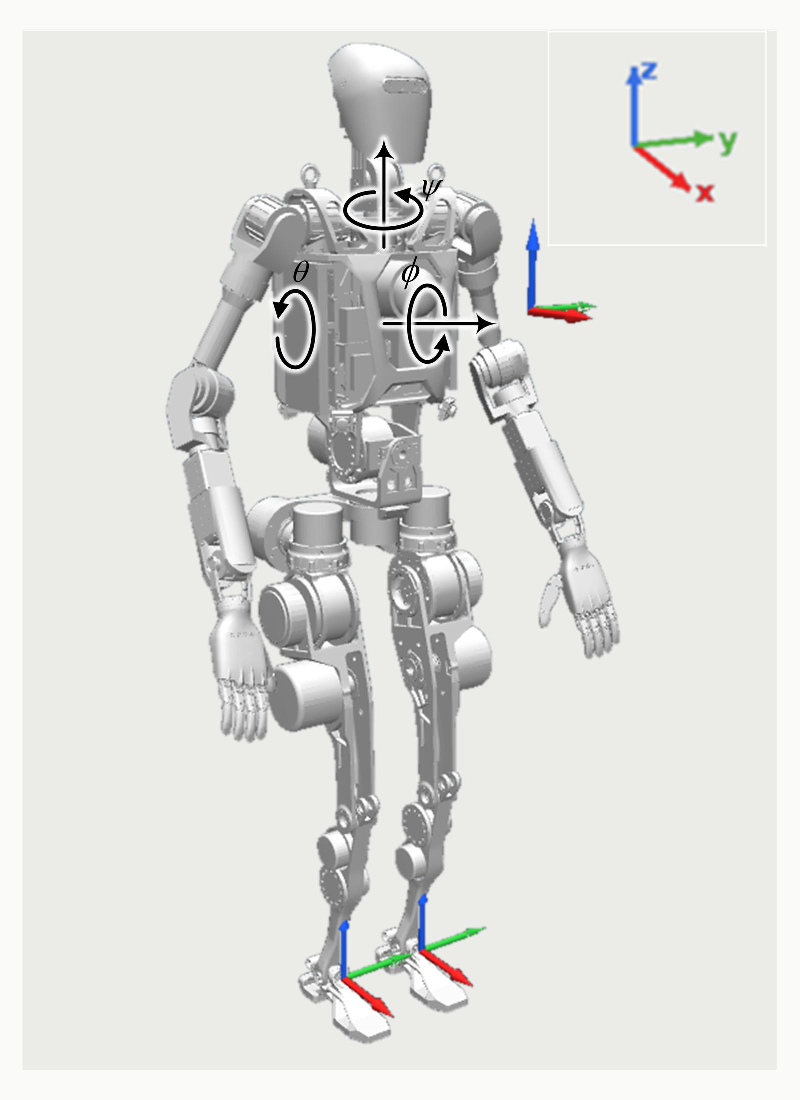
\includegraphics[height=8.2cm]{figures/manuscript_current/fig1_sign_conventions.pdf}
\caption{质心动力学模型中采用的世界坐标系方向、机身姿态符号以及足端接触力方向约定。}
\label{fig:sign_conventions}
\end{figure}
SRBM采用如下低维动力学近似：
\begin{equation}
m\ddot{\bm c}=\sum_{k=1}^{N_c}\bm f_k+m\bm g,
\label{eq:srbm_lin}
\end{equation}
\begin{equation}
\dot{\bm h}_G=\sum_{k=1}^{N_c}(\bm p_k-\bm c)\times \bm f_k+\sum_{k=1}^{N_c}\bm\tau_k,\quad
\bm h_G\simeq\bm I_0\bm\omega.
\label{eq:srbm_ang}
\end{equation}
其中，$\bm h_G$表示系统关于质心的角动量。式\eqref{eq:srbm_lin}--\eqref{eq:srbm_ang}表明，传统SRBM将整机关于质心的转动惯量近似为常值张量$\bm I_0$，从而能够以低维形式描述接触力/力矩与质心平动、转动动力学之间的关系，适合于高频凸优化求解；然而在双足机器人出现大幅摆腿、高速跨步或快速姿态调节时，摆动肢体会改变整机惯量分布，使$\bm I_0$不再能够准确刻画角动量演化。

为描述这种构型相关效应，本文引入整机关于系统质心的复合转动惯量$\bm I_G(\bm q)\in\mathbb{R}^{3\times3}$。根据质心动量表示，系统关于质心的角动量可写成与机身角速度相关的惯量项和与关节相对运动相关的剩余项之和。将该剩余项记为$\bm h_{\mathrm{rel}}(\bm q,\dot{\bm q}_j)$，则有
\begin{equation}
\bm h_G
=\bm I_G(\bm q)\bm\omega+\bm h_{\mathrm{rel}}(\bm q,\dot{\bm q}_j)
\simeq \bm I_G(\bm q)\bm\omega ,
\label{eq:IG}
\end{equation}
其中，$\dot{\bm q}_j$表示关节速度。本文的低维MPC预测状态仅包含机身姿态、质心位置、机身角速度和质心速度，并不显式预测未来关节速度及摆动腿相对运动。因此，在预测模型中忽略$\bm h_{\mathrm{rel}}$及其时间导数，得到式\eqref{eq:IG}中的近似表达；该近似保留$\bm I_G(\bm q)$随当前构型变化所反映的质量分布效应。

在计算上，本文利用centroidal composite rigid-body algorithm在线获得$\bm I_G(\bm q)$。该算法沿机器人树结构递推聚合各支链刚体惯量，从而高效获得整机惯量及其质心相关量\cite{ref44,ref80}；除该类递推算法外，也可通过传统的刚体惯量累加或基于雅可比矩阵的动能等效方法求取对应的质心惯量。由于$\bm I_G(\bm q)$随构型变化实时更新，它能够显式反映摆动肢体对整机惯量分布的影响。记外部接触扳手关于质心产生的合力矩为
\begin{equation}
\bm\tau_{\text{ext}}
=\sum_{k=1}^{N_c}(\bm p_k-\bm c)\times \bm f_k+\sum_{k=1}^{N_c}\bm\tau_k .
\label{eq:tau_ext}
\end{equation}
式\eqref{eq:tau_ext}中的$\bm\tau_{\text{ext}}$与式\eqref{eq:srbm_ang}右端的合力矩含义相同，均表示所有外部接触扳手关于系统质心产生的总力矩。其中，$(\bm p_k-\bm c)\times \bm f_k$为第$k$个接触力对质心的力矩，$\bm\tau_k$为该接触点直接施加的接触力矩；后文引入$\bm\tau_{\text{ext}}$只是为了简化记号，并不表示额外的控制输入。
由角动量平衡关系$\dot{\bm h}_G=\bm\tau_{\text{ext}}$，并对式\eqref{eq:IG}中的低维近似角动量求导，可得
\begin{equation}
\bm\tau_{\text{ext}}
=\dot{\bm h}_G
\simeq
\bm I_G(\bm q)\dot{\bm\omega}
+\dot{\bm I}_G\bm\omega .
\label{eq:hGdot}
\end{equation}
其中，$\dot{\bm I}_G\bm\omega$表示由系统构型变化导致的角动量变化项。式\eqref{eq:hGdot}仍是面向低维预测模型的近似表达，其忽略项主要来自$\dot{\bm h}_{\mathrm{rel}}$以及预测域内未显式建模的摆动腿相对动力学。由此可得角速度动力学近似为
\begin{equation}
\dot{\bm\omega}
\simeq
\bm I_G^{-1}\bm\tau_{\text{ext}}
-\bm I_G^{-1}\dot{\bm I}_G\bm\omega .
\label{eq:ang_dyn}
\end{equation}
与传统SRBM相比，式\eqref{eq:ang_dyn}的关键变化在于：预测模型的转动惯量不再固定，而是随关节构型在线更新；同时，惯量变化项作为角速度状态的线性项进入局部预测模型。为了与力/力矩驱动的MPC结构保持一致，定义状态和输入向量为\begin{equation}
\bm x=\begin{bmatrix}\bm\Theta^\top&\bm c^\top&\bm\omega^\top&\bm v^\top\end{bmatrix}^\top,\quad
\bm u=\begin{bmatrix}\bm f_l^\top&\bm\tau_l^\top&\bm f_r^\top&\bm\tau_r^\top\end{bmatrix}^\top,\ \bm v=\dot{\bm c}.
\label{eq:state_input}
\end{equation}
\begin{figure}[t]
\centering
\begin{minipage}[t]{0.48\linewidth}
\centering
\figplaceholder{figures/manuscript_current/fig1b_srbm_definition.pdf}{0.98\linewidth}{5.8cm}
\par\vspace{1mm}
{\small (a)}
\end{minipage}\hfill
\begin{minipage}[t]{0.48\linewidth}
\centering
\figplaceholder{figures/manuscript_current/fig1c_vicm_definition.pdf}{0.98\linewidth}{5.8cm}
\par\vspace{1mm}
{\small (b)}
\end{minipage}
\caption{SRBM与VICM的概念对比：(a) SRBM将机器人近似为具有常值质心惯量的单刚体，并采用腿部惯量较小的近似假设；(b) VICM在线更新构型相关质心惯量，并在质心预测模型中表征腿部运动引起的惯量变化。}
\label{fig:model_concepts}
\end{figure}
其中，$\bm\Theta=[\phi,\theta,\psi]^\top$表示机身姿态角，$\bm f_l,\bm f_r$与$\bm\tau_l,\bm\tau_r$分别为左右足的接触力与接触力矩。它们与式\eqref{eq:srbm_lin}--\eqref{eq:srbm_ang}中的通用接触力$\bm f_k$和接触力矩$\bm\tau_k$之间的关系为
\begin{equation}
(\bm p_1,\bm f_1,\bm\tau_1)=(\bm p_l,\bm f_l,\bm\tau_l),\qquad
(\bm p_2,\bm f_2,\bm\tau_2)=(\bm p_r,\bm f_r,\bm\tau_r).
\label{eq:contact_lr_mapping}
\end{equation}
也就是说，式\eqref{eq:state_input}只是将式\eqref{eq:srbm_lin}--\eqref{eq:srbm_ang}中的接触项按左、右足顺序展开为MPC输入；当某只脚处于摆动相时，对应足端接触力和接触力矩由接触时序约束为零。为说明预测矩阵的来源，定义
\begin{equation}
\bm r_i=\bm p_i-\bm c,\qquad
\bm S(\bm r_i)\bm f_i=\bm r_i\times\bm f_i,\quad i\in\{l,r\},
\label{eq:ri_skew}
\end{equation}
其中，$\bm S(\cdot)$为叉乘矩阵。考虑质心平动方程、姿态运动学关系以及式\eqref{eq:ang_dyn}，并在当前姿态、接触几何和构型相关惯量附近进行局部线性化，可得
\begin{equation}
\begin{aligned}
\dot{\bm\Theta}&\simeq \bm R_z^\top\bm\omega,\\
\dot{\bm c}&=\bm v,\\
\dot{\bm\omega}
&\simeq\bm I_G^{-1}\!\left[
\bm S(\bm r_l)\bm f_l+\bm\tau_l
+\bm S(\bm r_r)\bm f_r+\bm\tau_r
\right]
-\bm I_G^{-1}\dot{\bm I}_G\bm\omega,\\
\dot{\bm v}&=\frac{1}{m}(\bm f_l+\bm f_r)+\bm g .
\end{aligned}
\label{eq:continuous_blocks}
\end{equation}
式\eqref{eq:continuous_blocks}第一行采用仅含yaw角的小roll/pitch近似，将世界系机身角速度映射为roll-pitch-yaw角速度。在该近似下，roll和pitch角速度仍通过$\bm R_z^\top\bm\omega$的水平分量保留，高阶roll-pitch耦合项被忽略。式\eqref{eq:continuous_blocks}将姿态运动学、质心平动动力学和质心角动力学分别写成与状态、接触扳手和仿射项相关的分块形式。将各项按式\eqref{eq:state_input}的状态与输入顺序整理，可得到连续时间仿射模型
\begin{equation}
\dot{\bm x}=\bm A_c\bm x+\bm B_c(\bm q)\bm u+\bm g_c(\bm q,\dot{\bm q}),
\label{eq:affine}
\end{equation}
其分块形式写为\begin{equation}
\bm A_c=
\begin{bmatrix}
\bm 0 & \bm 0 & \bm R_z^\top & \bm 0\\
\bm 0 & \bm 0 & \bm 0 & \bm I\\
\bm 0 & \bm 0 & -\bm I_G^{-1}\dot{\bm I}_G & \bm 0\\
\bm 0 & \bm 0 & \bm 0 & \bm 0
\end{bmatrix},
\label{eq:Ac}
\end{equation}
\begin{equation}
\bm B_c=
\begin{bmatrix}
\bm 0 & \bm 0 & \bm 0 & \bm 0\\
\bm 0 & \bm 0 & \bm 0 & \bm 0\\
\bm I_G^{-1}\bm S(\bm r_l) & \bm I_G^{-1} & \bm I_G^{-1}\bm S(\bm r_r) & \bm I_G^{-1}\\
\frac{1}{m}\bm I & \bm 0 & \frac{1}{m}\bm I & \bm 0
\end{bmatrix},
\label{eq:Bc}
\end{equation}
\begin{equation}
\bm g_c=
\begin{bmatrix}
\bm 0\\ \bm 0\\ \bm 0\\ \bm g
\end{bmatrix}.
\label{eq:gc}
\end{equation}
其中，$\bm R_z(\psi)$表示由当前机身偏航角构造的yaw旋转矩阵，$\bm I$为三维单位矩阵。由式\eqref{eq:Ac}--\eqref{eq:gc}可见，$\bm A_c$由姿态运动学、质心位置积分关系以及惯量变化项共同决定，$\bm B_c$由接触力/力矩对质心角加速度和线加速度的贡献决定，而$\bm g_c$收集重力项。SRBM可视为该模型的特例，即令$\bm I_G(\bm q)=\bm I_0$且$\dot{\bm I}_G=\bm 0$；VICM则在保持相同状态维度和输入维度的同时，通过实时更新$\bm I_G(\bm q)$和$\dot{\bm I}_G$实现对摆动肢体惯性影响的显式刻画。工程实现中，$\dot{\bm I}_G$由相邻控制周期的$\bm I_G(\bm q)$有限差分估计。由于有限差分对构型测量噪声和数值误差较敏感，本文在将$\dot{\bm I}_G$用于MPC状态矩阵前施加一阶低通滤波；该处理仅作为惯量导数估计的数值平滑步骤，不改变式\eqref{eq:ang_dyn}所示的动力学模型形式。SRBM与VICM在惯量建模方式上的核心差异如图~\ref{fig:model_concepts}所示。这也为后续构建兼顾实时性与保真度的MPC优化问题提供了统一动力学基础。
\section{Controller Design}
本节基于第2节建立的低维质心动力学模型，给出完整闭环控制器的实现方式。整体行走控制栈基于OpenLoong Dynamics Control开源框架实现\cite{refOpenLoong}；本文在该框架上修改质心预测模型与MPC动力学项。控制器由三部分组成：首先，MPC在有限预测域内优化支撑足接触扳手；其次，摆动腿规划模块根据速度指令与当前步态相位生成落脚点和足端轨迹；最后，WBC将高层接触扳手和运动参考映射为满足全身动力学与接触约束的关节力矩。

\subsection{MPC Controller Design}
本文采用“高层质心MPC + 低层WBC”的分层控制架构。高层控制器基于第2节建立的变惯量质心模型，在有限预测域内优化接触力与接触力矩；低层控制器则在全身动力学与接触约束下，将这些高层决策映射为可执行的关节加速度和关节力矩。沿用现有centroidal MPC方案中常见的 receding-horizon 处理方式，对连续时间模型的状态与输入映射部分按照MPC离散化周期$\Delta t_{\mathrm{mpc}}$进行离散化。考虑到控制周期较短，本文采用前向Euler方法，即
\begin{equation}
\bm A_k=\bm I+\Delta t_{\mathrm{mpc}}\bm A_c(k),\qquad
\bm B_k=\Delta t_{\mathrm{mpc}}\bm B_c(k),\qquad
\bm c_k=\Delta t_{\mathrm{mpc}}\bm c_c(k),
\label{eq:euler_disc}
\end{equation}
其中，$\bm A_c(k)$和$\bm B_c(k)$分别表示第$k$个预测节点处由当前姿态、接触几何及构型相关惯量线性化得到的连续时间系统矩阵与输入矩阵；$\bm c_c(k)$表示实现中保留的剩余仿射偏置项。由此可得离散时间预测模型\begin{equation}
\bm x_{k+1}=\bm A_k\bm x_k+\bm B_k\bm u_k+\bm c_k.
\label{eq:disc}
\end{equation}
其中，$N_p$表示预测域内的离散预测状态节点数，物理预测时长为$T_p=N_p\Delta t_{\mathrm{mpc}}$；$N_u$表示优化输入的控制域长度。本文实现中取$N_u<N_p$，预测矩阵在控制域之后保持最后一个优化输入块不变。每个控制周期内，MPC基于当前测得状态$\bm x_0$求解控制域内的最优接触扳手序列$\{\bm u_0^\ast,\bm u_1^\ast,\ldots,\bm u_{N_u-1}^\ast\}$；实际执行时仅施加当前时刻控制量$\bm u_0^\ast$，随后预测域向前滚动一个采样周期，并利用更新后的状态重新构造和求解优化问题。该 receding-horizon 机制使得控制器能够持续修正模型误差、状态漂移以及外部扰动对系统演化的影响。MPC以预测状态跟踪与控制正则化为目标，构造代价函数\begin{equation}
\displaystyle
\min_{\bm U} J=\sum_{k=1}^{N_p}\|\bm x_k-\bm x_k^{\text{ref}}\|_{\bm Q}^2+
\alpha\sum_{j=0}^{N_u-1}\|\bm u_j-\bar{\bm u}_j\|_{\bm R}^2
\label{eq:cost}
\end{equation}
其中，$\bm x_k^{\text{ref}}$为质心、姿态及角速度参考轨迹，$\bar{\bm u}_j$表示名义接触扳手正则化中心，$\bm Q$和$\bm R$分别为状态和控制量权重矩阵，$\alpha$为输入正则化系数。$\bar{\bm u}_j$为输入正则化项提供名义载荷分配基准；实现中，名义重力载荷分配由该正则化中心给出，离散预测模型中的剩余仿射偏置由$\bm c_k$表示。第$j$个控制节点的名义接触扳手中心取为
\begin{equation}
\begin{aligned}
&\bar{\bm u}_j=
\begin{bmatrix}
\bar{\bm f}_{l,j}^{\top}&\bm 0_3^{\top}&
\bar{\bm f}_{r,j}^{\top}&\bm 0_3^{\top}
\end{bmatrix}^{\top},
\\
&\bar{\bm f}_{l,j}=
-\gamma_{l,j}m\bm g,
\\
&\bar{\bm f}_{r,j}=
-\gamma_{r,j}m\bm g,
\end{aligned}
\label{eq:nominal_wrench}
\end{equation}
其中，$(\gamma_{l,j},\gamma_{r,j})$由步态相位确定：左支撑时为$(1,0)$，右支撑时为$(0,1)$，双支撑时为$(1/2,1/2)$。具体实现中，MPC使用的支撑腿状态和步态相位由步态调度器更新，步态调度器通过比较足底垂向力反馈$F_{z,l}$、$F_{z,r}$与预设接触阈值判断支撑腿切换。为简化表示，本文将由此得到的步态/接触状态记为$\chi_g$，其包含MPC和WBC使用的当前支撑腿、摆动腿和步态相位信息。用户层给定的速度指令$v_x^{\mathrm{cmd}}$、$v_y^{\mathrm{cmd}}$和$\omega_z^{\mathrm{cmd}}$首先经斜坡生成、航向积分和坐标变换得到当前期望状态采样点$\bm x_d(t)$，其包含期望姿态、质心位置、角速度和线速度。MPC内部通过滚动更新方式将连续生成的$\bm x_d(t)$组织为预测域内的堆叠状态参考。接触扳手$\bm u_j$为MPC优化变量，$\bar{\bm u}_j$按步态相位和名义重力载荷分配设置。

设第$n$个MPC更新时刻生成的当前期望状态采样点为$\bm r_n=\bm x_d(t_n)$。MPC内部维护堆叠参考向量
\begin{equation}
\bm X_d^{(n)}
=
\begin{bmatrix}
(\bm x_{1}^{\text{ref},(n)})^\top &
(\bm x_{2}^{\text{ref},(n)})^\top &
\cdots &
(\bm x_{N_p}^{\text{ref},(n)})^\top
\end{bmatrix}^{\top}.
\label{eq:rolling_ref}
\end{equation}
在每次更新时，该向量先向前滚动一位，并将最新参考采样点$\bm r_n$填入末端，即
\begin{equation}
\bm X_d^{(n)}
=
\begin{bmatrix}
(\bm x_{2}^{\text{ref},(n-1)})^\top &
\cdots &
(\bm x_{N_p}^{\text{ref},(n-1)})^\top &
\bm r_n^\top
\end{bmatrix}^{\top}.
\label{eq:rolling_ref_update}
\end{equation}
因此，代价函数中的$\bm x_k^{\text{ref}}$表示$\bm X_d$中的第$k$个状态参考块。将预测域内的状态和控制量沿时间轴堆叠为
\begin{equation}
\bm X=
\begin{bmatrix}
\bm x_1^\top & \bm x_2^\top & \cdots & \bm x_{N_p}^\top
\end{bmatrix}^\top,\qquad
\bm U=
\begin{bmatrix}
\bm u_0^\top & \bm u_1^\top & \cdots & \bm u_{N_u-1}^\top
\end{bmatrix}^\top,
\label{eq:stack}
\end{equation}
则式\eqref{eq:disc}可进一步写成全视界的紧凑形式为\begin{equation}
\bm X=\bar{\bm A}\bm x_0+\bar{\bm B}\bm U+\bar{\bm C},
\label{eq:predcompact}
\end{equation}
其中，$\bar{\bm A},\bar{\bm B},\bar{\bm C}$分别为由离散系统矩阵递推得到的状态转移矩阵、输入映射矩阵与仿射项堆叠矩阵，$\bm x_0$为当前时刻测得的系统状态。为说明式\eqref{eq:cost}到二次规划的转换，定义
\begin{equation}
\begin{aligned}
\bm X_d&=\begin{bmatrix}(\bm x_1^{\text{ref}})^\top&\cdots&(\bm x_{N_p}^{\text{ref}})^\top\end{bmatrix}^{\top},\\
\bar{\bm U}&=\begin{bmatrix}\bar{\bm u}_0^\top&\cdots&\bar{\bm u}_{N_u-1}^\top\end{bmatrix}^{\top},
\end{aligned}
\label{eq:stacked_ref_input}
\end{equation}
并令$\bar{\bm Q}=\mathrm{diag}(\bm Q,\ldots,\bm Q)$、$\bar{\bm R}=\mathrm{diag}(\bm R,\ldots,\bm R)$。则式\eqref{eq:cost}可写为
\begin{equation}
J=(\bm X-\bm X_d)^\top\bar{\bm Q}(\bm X-\bm X_d)
+\alpha(\bm U-\bar{\bm U})^\top\bar{\bm R}(\bm U-\bar{\bm U}).
\label{eq:stacked_cost}
\end{equation}
将式\eqref{eq:predcompact}代入，并记$\bm e_0=\bar{\bm A}\bm x_0+\bar{\bm C}-\bm X_d$，可得
\begin{equation}
\scalebox{0.92}{$
J=\bm U^\top(\bar{\bm B}^\top\bar{\bm Q}\bar{\bm B}+\alpha\bar{\bm R})\bm U
+2(\bar{\bm B}^\top\bar{\bm Q}\bm e_0-\alpha\bar{\bm R}\bar{\bm U})^\top\bm U.
$}
\label{eq:expanded_cost}
\end{equation}
整理后即可得到标准二次规划形式\begin{equation}
\min_{\bm U}\ \frac{1}{2}\bm U^\top \bm H\bm U+\bm c^\top\bm U
\quad
\text{s.t.}\quad
\bm A_{\text{ineq}}\bm U\le \bm b_{\text{ineq}},\ \
\bm U_{\min}\le \bm U\le \bm U_{\max},
\label{eq:qpcompact}
\end{equation}
其中，$\bm H=2(\bar{\bm B}^\top\bar{\bm Q}\bar{\bm B}+\alpha\bar{\bm R})$为由权重矩阵诱导的半正定Hessian矩阵，$\bm c=2(\bar{\bm B}^\top\bar{\bm Q}\bm e_0-\alpha\bar{\bm R}\bar{\bm U})$为与参考轨迹、当前状态和名义接触扳手有关的线性项。该二次规划在每个预测节点均需满足接触扳手可行性与步态相位约束。对任一处于支撑相的足端，摩擦锥近似约束写为
\begin{equation}
|f_{x,i}|\le \mu f_{z,i},\qquad |f_{y,i}|\le \mu f_{z,i}.
\label{eq:c_fric}
\end{equation}
其中，$f_x,f_y,f_z$分别表示局部足端坐标系下的切向力和法向力，$\mu$为摩擦系数。单边接触条件进一步要求为\begin{equation}
f_{z,\min}\le f_{z,i}\le f_{z,\max}.
\label{eq:c_normal}
\end{equation}
为保证压力中心位于支撑域内部，足端接触力矩需满足
\begin{equation}
-d_y^- f_{z,i}\le \tau_{x,i}\le d_y^+ f_{z,i}.
\label{eq:c_copx}
\end{equation}
\begin{equation}
-d_x^- f_{z,i}\le \tau_{y,i}\le d_x^+ f_{z,i}.
\label{eq:c_copy}
\end{equation}
其中，$\tau_x,\tau_y$表示局部足端坐标系下的接触力矩分量，$d_x^\pm,d_y^\pm$表示足底中心到边界的几何距离参数。优化变量还需满足输入边界
\begin{equation}
\bm u_{\min}\le \bm u_k\le \bm u_{\max}.
\label{eq:c_bound}
\end{equation}
对于单支撑阶段的摆动足，还需施加零接触等式约束\begin{equation}
\bm f_{\text{sw},k}=\bm 0,\qquad \bm\tau_{\text{sw},k}=\bm 0.
\label{eq:c_swing}
\end{equation}
其中，下标$i$表示预测域内统一编号后的接触扳手变量分量，下标$k$表示离散时刻，$\text{sw}$表示摆动足。将式\eqref{eq:c_fric}--\eqref{eq:c_swing}沿预测域展开后，可统一写成式\eqref{eq:qpcompact}中的线性不等式和边界约束。求解得到的第一步最优接触扳手作为当前控制周期的高层输出发送至低层WBC执行。
\subsection{Swing Leg Trajectory Generation}
在MPC主要负责支撑足扳手分配的同时，摆动足轨迹由独立的步态规划模块生成。类似于经典Raibert足式控制思想及后续双足步态规划工作\cite{ref63,ref79}，本文采用“Raibert落脚点规划 + 摆线插值”的两级结构：前者根据用户速度指令、当前质心速度与当前步态相位给出水平落脚点，后者生成满足起落点速度连续的摆动轨迹。Raibert型落脚点规划写为\begin{equation}
\bm p_{\text{des}}
=\bm p_{\text{hip}}
-\bm K_v(\bm v_{xy}^{\mathrm{cmd}}-\bm v_{xy})
+\frac{T_{\text{sw}}}{2}\bm v_{xy}
+(1-\phi)T_{\text{sw}}\bm v_{xy}.
\label{eq:raibert}
\end{equation}
其中，$\bm p_{\text{des}}$为期望落脚点，$\bm p_{\text{hip}}$为髋关节投影位置，$\bm v_{xy}$为状态向量中质心速度$\bm v$的水平分量，$\bm v_{xy}^{\mathrm{cmd}}=[v_x^{\mathrm{cmd}},\,v_y^{\mathrm{cmd}},\,0]^\top$由用户层水平速度指令组成，$\bm K_v$为速度反馈增益矩阵，$T_{\text{sw}}$为摆动相持续时间，$\phi$为摆动相位变量。具体实现中，Raibert落脚点仅使用水平速度误差反馈，其增益矩阵写为
\begin{equation}
\bm K_v
=\bm R_z(\psi)
\begin{bmatrix}
k_{p,v_x} & 0 & 0\\
0 & k_{p,v_y} & 0\\
0 & 0 & 0
\end{bmatrix}
\bm R_z^\top(\psi),
\label{eq:swing_kv}
\end{equation}
其中，$\psi$为当前基座偏航角，$\bm R_z(\psi)$用于将机身对齐坐标系下的水平反馈增益映射至世界坐标系。增益$k_{p,v_x}$与$k_{p,v_y}$的具体数值见表~\ref{tab:swing_param}。对转向步态，进一步引入偏航修正\begin{equation}
\Delta \bm p_{\text{yaw}}
=\frac{w_{\text{hip}}}{2}
\begin{bmatrix}
\cos\theta_f-\cos\theta_0\\
\sin\theta_f-\sin\theta_0\\
0
\end{bmatrix},
\end{equation}
\begin{equation}
\theta_f=\theta_0+\omega_z(1-\phi)T_{\text{sw}}+\frac{1}{2}\omega_zT_{\text{sw}}+k_{p,\omega_z}(\omega_z-\omega_z^{\mathrm{cmd}}).
\label{eq:yaw}
\end{equation}
其中，$w_{\text{hip}}$为两髋横向间距，$\theta_0$与$\theta_f$分别为当前和预测偏航角，$\omega_z$为状态向量中角速度$\bm\omega$的偏航分量，$\omega_z^{\mathrm{cmd}}$为用户层偏航角速度指令，$k_{p,\omega_z}$为偏航反馈增益。给定落脚点后，摆动相插值函数取为\begin{equation}
s(\phi)=\phi-\frac{\sin(2\pi\phi)}{2\pi},
\label{eq:phase}
\end{equation}
则水平和竖直方向的摆动轨迹分别写为\begin{equation}
\bm p_{xy}^{\text{sw}}(\phi)=\bm p_{xy}^{0}+s(\phi)\left(\bm p_{xy}^{f}-\bm p_{xy}^{0}\right),
\label{eq:trajxy}
\end{equation}
\begin{equation}
z^{\text{sw}}(\phi)=z_0+\frac{h}{2}\left(1-\cos 2\pi\phi\right)+s(\phi)(z_f-z_0).
\label{eq:trajz}
\end{equation}
式\eqref{eq:trajz}中，$h$对应摆动足抬脚高度$H_{\mathrm{step}}$。终端足高根据控制器中的名义站立腿长与足端离地高度补偿生成，使平地行走时的足端目标与期望基座高度保持一致。上述规划在起跳与触地时刻保持速度连续，可减小接触切换瞬间的冲击。

\begin{table}[t]
\centering
\caption{摆动腿规划主要参数}
\label{tab:swing_param}
\footnotesize
\begin{tabular*}{\linewidth}{@{\extracolsep{\fill}}L{0.48\linewidth}L{0.24\linewidth}L{0.18\linewidth}@{}}
\hline
参数 & 符号/单位 & 数值 \\
\hline
摆动腿速度反馈增益$x$向 & $k_{p,v_x}$ & 0.10 \\
摆动腿速度反馈增益$y$向 & $k_{p,v_y}$ & 0.03 \\
偏航反馈增益 & $k_{p,\omega_z}$ & 0.03 \\
摆动相持续时间 & $T_{\mathrm{sw}}$/s & 0.45（实验一、三、四） \\
 & & 0.25（实验二） \\
摆动腿抬脚高度 & $H_{\mathrm{step}}$/m & 0.205 \\
足端离地高度补偿 & $h_{\mathrm{foot}}$/m & 0.07 \\
名义站立腿长 & $L_{\mathrm{leg}}$/m & 1.05 \\
髋间距 & $w_{\mathrm{hip}}$/m & 0.209 \\
\hline
\end{tabular*}
\end{table}

\subsection{WBC Controller Design}
WBC层采用广泛使用的“centroidal MPC + inverse-dynamics QP”低层实现形式\cite{ref36,ref55,ref63}，在高频控制层恢复全身动力学可行性、满足接触一致性并执行摆动腿与躯干任务。其基本动力学约束为\begin{equation}
\bm M(\bm q)\ddot{\bm q}
+\bm C(\bm q,\dot{\bm q})\dot{\bm q}
+\bm G(\bm q)
=\bm S^\top\bm\tau_j+\bm J_c^\top\bm f,
\label{eq:wbcdyn}
\end{equation}
\begin{equation}
\bm J_c\ddot{\bm q}+\dot{\bm J}_c\dot{\bm q}=\bm 0.
\label{eq:wbccontact}
\end{equation}
式\eqref{eq:wbcdyn}给出全身逆动力学平衡关系，式\eqref{eq:wbccontact}要求处于支撑相的接触点满足刚性接触加速度约束。高层MPC给出的左右足接触力$\bm f_l,\bm f_r$与任务层根据支撑接触、躯干调节和摆动足跟踪生成的期望广义加速度$\ddot{\bm q}_{\text{ref}}$共同构成WBC参考输入。在该参考输入基础上，低层逆动力学QP进一步求解满足式\eqref{eq:wbcdyn}、式\eqref{eq:wbccontact}及接触力可行域约束的最小修正量，即
\begin{equation}
\min_{\delta\ddot{\bm q},\delta\bm f,\bm\tau_j}
\left\|\delta\ddot{\bm q}\right\|^2
+\left\|\delta\bm f\right\|^2
+\left\|\bm\tau_j\right\|^2
\label{eq:wbcqp}
\end{equation}
并满足\begin{equation}
\ddot{\bm q}=\ddot{\bm q}_{\text{ref}}+\delta\ddot{\bm q},\qquad
\bm f=\begin{bmatrix}\bm f_l^\top&\bm f_r^\top\end{bmatrix}^\top+\delta\bm f,
\end{equation}
\begin{equation}
\bm\tau_{j,\min}\le \bm\tau_j\le \bm\tau_{j,\max},\qquad \bm f\in\mathcal{K}_\mu.
\label{eq:wbcbound}
\end{equation}
其中，$\delta\ddot{\bm q}$与$\delta\bm f$分别表示对参考加速度和参考接触力的修正量，$\mathcal{K}_\mu$表示线性化摩擦锥可行域。低层WBC在高层MPC给出的期望接触扳手与任务层生成的运动参考基础上，联合求解满足动力学与接触约束的广义加速度$\ddot{\bm q}$、接触力$\bm f$和关节驱动力矩$\bm\tau_j$。具体实现中，WBC输出被转换为关节位置参考$\bm q^{\mathrm{des}}$、关节速度参考$\dot{\bm q}^{\mathrm{des}}$和关节力矩前馈$\bm\tau_j^{\mathrm{ff}}$，并输入关节级位置-速度-力矩（Position-Velocity-Torque, PVT）控制器，由该控制器生成发送至仿真机器人的最终电机力矩$\bm\tau^{\mathrm{out}}$。WBC任务包括支撑接触一致性、躯干姿态与位置调节、摆动腿轨迹跟踪以及上肢和冗余关节调节等。由于本文关注高层预测模型差异，WBC任务结构和参数在所有对比实验中保持一致，仅作为统一的全身动力学执行层。综上，MPC、摆动腿规划、WBC与机器人本体之间的信息流如图~\ref{fig:control_framework}所示，其中用户速度指令经参考生成模块进入MPC与落脚点规划，MPC输出的接触扳手和任务层运动参考共同构成WBC的输入。
\begin{figure}[t]
\centering
\figplaceholder{figures/manuscript_current/fig3.jpg}{0.88\linewidth}{5.3cm}
\caption{整体控制框架示意图。}
\label{fig:control_framework}
\end{figure}
\section{Simulation and Performance Comparison}
本节通过MuJoCo全身动力学仿真评估所提VICM-MPC与SRBM-MPC在不同工况下的表现。首先给出仿真环境、机器人参数和统一控制参数；随后设计腿部惯量扫描、名义速度跟踪、模型结构消融和外部扰动恢复四类实验；最后从survival time、跟踪曲线、消融结果、扰动恢复区域以及在线计算时间等方面进行对比分析。

\subsection{Simulation Setup and Robot Parameters}
本文在MuJoCo全身动力学仿真平台上完成所有对比实验，并采用Pinocchio进行运动学与动力学计算，从而保证仿真中的状态反馈、接触信息与控制器内部建模保持一致。机器人在平地行走中的代表性仿真快照如图~\ref{fig:walking_snapshots}所示，与控制代码对应的主要仿真环境参数列于表~\ref{tab:sim_param}。

\begin{figure}[t]
\centering
\figplaceholder{figures/manuscript_current/fig4_walking_snapshots.png}{0.86\linewidth}{5.2cm}
\caption{机器人在MuJoCo仿真环境中的代表性平地行走快照。前三帧采样于起步双支撑阶段，其余帧展示随后进入单支撑后的行走过程。图中标签分别表示双支撑、左支撑和右支撑阶段，白色虚线表示支撑相切换位置。}
\label{fig:walking_snapshots}
\end{figure}

\begin{table}[t]
\centering
\caption{仿真环境主要参数}
\label{tab:sim_param}
\begin{tabular*}{\linewidth}{@{\extracolsep{\fill}}lcc}
\hline
参数 & 符号/单位 & 数值 \\
\hline
仿真器 & -- & MuJoCo \\
运动学/动力学库 & -- & Pinocchio \\
动力学积分步长 & $\Delta t_{\mathrm{sim}}$/s & 0.001 \\
WBC更新周期 & $\Delta t_{\mathrm{wbc}}$/s & 0.001 \\
MPC更新周期 & $\Delta t_{\mathrm{mpc}}$/s & 0.005 \\
重力加速度 & $\bm g$/m$\cdot$s$^{-2}$ & $[0,0,-9.81]^\top$ \\
预测域长度 & $N_p$ & 10 \\
有效预测时长 & $N_p\Delta t_{\mathrm{mpc}}$/s & 0.05 \\
控制域长度 & $N_u$ & 3 \\
地面摩擦系数 & $\mu$ & 0.5 \\
最长仿真时长 & $T_{\mathrm{sim}}$/s & 30 \\
\hline
\end{tabular*}
\end{table}

需要说明的是，预测域内的$\bm I_G(\bm q)$和$\dot{\bm I}_G$采用当前控制周期测得构型处的局部线性化值，并随滚动时域在下一控制周期重新计算。本文取$N_p=10$时，有效预测时长为0.05 s。

被测对象为AzureLoong全身模型，其质量参数、惯性参数和关节布局均与控制代码所调用的URDF模型保持一致，表中几何尺寸由仿真所用MJCF/URDF模型提取得到。表~\ref{tab:robot_param}给出仿真模型的主要机器人参数。

\begin{table}[t]
\centering
\caption{机器人主要参数}
\label{tab:robot_param}
\footnotesize
\begin{tabular*}{\linewidth}{@{\extracolsep{\fill}}L{0.40\linewidth}L{0.25\linewidth}L{0.27\linewidth}@{}}
\hline
参数 & 符号/单位 & 数值 \\
\hline
机器人模型 & -- & AzureLoong全身模型 \\
总质量 & $m$/kg & 77.35 \\
身体/非腿部质量 & $M_b^0$/kg & 47.48 \\
双腿总质量 & $M_\ell^0$/kg & 29.87 \\
MJCF几何模型站立高度 & $H$/m & 1.818 \\
基座连杆外包围盒尺寸 & $l_b,w_b,h_b$/m & 0.297, 0.327, 0.540 \\
名义站立基座高度 & $H_b$/m & 1.12 \\
髋--膝与膝--踝偏置长度 & $l_1,l_2$/m & 0.400, 0.387 \\
足底碰撞盒尺寸 & $l_f,w_f,h_f$/m & 0.245, 0.080, 0.088 \\
URDF基座连杆惯量 & $(I_{xx},I_{yy},I_{zz})$/kg\,m$^2$ & 0.374, 0.277, 0.221 \\
URDF连杆数 & -- & 32 \\
URDF关节数 & -- & 31 \\
\hline
\end{tabular*}
\end{table}

此外，仿真中使用如下MPC权重矩阵：
\begin{equation}
\bm Q=\mathrm{diag}(50,50,80,\,1,200,1,\,1,1,10,\,100,10,1),
\end{equation}
\begin{equation}
\bm R=\bm I_{13},
\end{equation}
并取输入正则化系数$\alpha=10^{-6}$。其中，$\bm Q$对应式\eqref{eq:state_input}中状态向量的对角权重，分别作用于机身姿态、质心位置、角速度和质心线速度；$\bm R$对应接触扳手输入向量的对角权重。所有实验中的MPC权重、MPC约束参数、WBC参数、步态调度参数以及摆动腿规划参数均保持一致。

\subsection{Experimental Design}
本文设计四组对比实验，核心对比对象为采用常值惯量假设的单刚体模型控制器（SRBM-MPC）与采用构型相关惯量及惯量变化项的变惯量质心模型控制器（VICM-MPC）。除特别说明外，所有控制器共享相同的MPC权重、MPC约束、WBC执行层、WBC参数设置、摆动腿规划器和接触切换设置。步态切换采用触地检测信号，法向接触力阈值为100 N。VICM-MPC中的$\dot{\bm I}_G$由相邻控制周期的$\bm I_G$有限差分并经一阶低通滤波得到，滤波时间常数取0.01 s。

实验一用于分析摆动腿惯量增大后两类模型的稳定裕度差异。具体而言，本文通过腿部质量与转动惯量缩放系数$\lambda$构造不同程度的摆动惯量扰动，并在每个$\lambda$取值下施加相同的前向速度指令和正弦偏航角速度指令。$\lambda$取值为$1.0,1.1,\ldots,2.3$，即腿部质量与转动惯量相对于名义参数的1.0--2.3倍，步长为0.1；每个$\lambda$下SRBM-MPC和VICM-MPC均重复运行5次，单次仿真上限为30 s。前向速度指令为$v_x^{\mathrm{cmd}}=1.5$ m/s，摆动相持续时间为$T_{\mathrm{sw}}=0.45$ s。转向指令在$t<4$ s时为零，在$t\ge4$ s时取
\begin{equation}
\omega_z^{\mathrm{cmd}}(t)=0.25\sin\left(\frac{2\pi(t-4)}{4}\right)\ \mathrm{rad/s}.
\label{eq:exp_sine_wz}
\end{equation}
该实验的主要评价指标为survival time，即机器人在跌倒或失稳前能够维持运动的时间，并统计5次重复实验的均值和离散程度。通过扫描$\lambda$，可以观察当摆动肢体惯量提高且转向角动量变化增强时，SRBM与VICM在模型近似误差敏感性上的差异。

腿部惯量缩放的具体方式如下。设$\mathcal{L}$为左右腿连杆集合，包括左右髋、膝、踝相关连杆。对于每个腿部连杆$i\in\mathcal{L}$，本文按同一系数$\lambda$缩放其质量和转动惯量：
\begin{equation}
m_i(\lambda)=\lambda m_i^0,\qquad
\bm I_i(\lambda)=\lambda \bm I_i^0 ,
\label{eq:leg_lambda_scaling}
\end{equation}
其中，上标0表示URDF中的名义惯性参数。非腿部连杆惯性参数保持不变，因此整机总质量和腿部质量占比会随$\lambda$增大而提高。对应的双腿质量占比可写为
\begin{equation}
\rho_\ell(\lambda)=
\frac{\lambda M_\ell^0}{M^0+(\lambda-1)M_\ell^0},
\label{eq:leg_mass_fraction_lambda}
\end{equation}
其中，$M^0$为名义整机总质量，$M_\ell^0$为名义双腿总质量。根据URDF名义质量参数计算得到，机器人总质量为77.35 kg，左右腿连杆总质量为29.87 kg，对应名义双腿质量占比为0.386。通过这种方式，可以在不改变控制架构和步态规划器的前提下，系统考察摆动腿惯量变化对步态稳定性的影响。

实验二用于给出名义质量分布下的速度跟踪表现。该实验取$\lambda=1.0$，不引入转向目标，单次仿真时长为16 s，摆动相持续时间为$T_{\mathrm{sw}}=0.25$ s。前向速度实验中，侧向速度指令保持为零，前向速度指令在$t<8$ s时为0.6 m/s，在$8\le t\le11$ s内线性斜坡上升至1.2 m/s，并在$t>11$ s后保持1.2 m/s。侧向速度实验中，前向速度指令保持为零，侧向速度指令在$t<8$ s时为0.15 m/s，在$8\le t\le11$ s内线性斜坡上升至0.30 m/s，并在$t>11$ s后保持0.30 m/s。实验二展示SRBM-MPC与VICM-MPC的代表性速度响应曲线，用于说明双腿质量占比较低时两类低维模型均可嵌入同一MPC--WBC控制框架。

实验三用于分析VICM内部建模项对稳定性的贡献。该实验取$\lambda=1.7$，前向速度指令为$v_x^{\mathrm{cmd}}=1.5$ m/s，摆动相持续时间为$T_{\mathrm{sw}}=0.45$ s，偏航角速度指令与式\eqref{eq:exp_sine_wz}相同，单次仿真上限为30 s。每种模型变体重复运行3次。四种比较对象按图~\ref{fig:experiment3_ablation}中的顺序定义如下：SRBM采用常值惯量的单刚体模型；VICM为完整变惯量质心模型，在线更新构型相关惯量$\bm I_G(\bm q)$，将惯量变化项$-\bm I_G^{-1}\dot{\bm I}_G\bm\omega$纳入角速度状态矩阵，并对有限差分得到的$\dot{\bm I}_G$进行低通滤波；VICM-IG仅在线更新构型相关惯量$\bm I_G(\bm q)$，不使用惯量变化项$-\bm I_G^{-1}\dot{\bm I}_G\bm\omega$；VICM-NF与VICM采用相同模型形式，仍包含$-\bm I_G^{-1}\dot{\bm I}_G\bm\omega$，但关闭对有限差分$\dot{\bm I}_G$的一阶低通滤波。该消融实验用于区分构型相关惯量、惯量变化项以及数值平滑处理对闭环稳定性和角速度预测误差的影响。

实验四用于分析外部扰动作用下的步态恢复能力。该实验取$\lambda=1.7$，前向速度指令为$v_x^{\mathrm{cmd}}=1.2$ m/s，不施加转向指令，摆动相持续时间为$T_{\mathrm{sw}}=0.45$ s，单次仿真上限为15 s。水平脉冲扰动施加于机器人躯干。为避免固定绝对时间扰动恰好落在换腿边界，本文在$t\ge8$ s之后等待步态相位首次到达$\phi=0.5$时触发扰动，持续时间为0.15 s。扰动方向角$\theta_F$取$0^\circ,45^\circ,\ldots,315^\circ$，扰动力幅值取$0,100,200,300,400$ N；每个方向和幅值组合分别对SRBM-MPC与VICM-MPC重复运行5次。该实验统计机器人是否能够在扰动后维持至仿真结束，并绘制方向--幅值恢复区域图和代表性扰动响应曲线。

综上，实验一采用重复运行统计模型在不同腿部惯量下的稳定裕度；实验二展示名义速度跟踪曲线；实验三整理为模型结构消融对比；实验四整理为扰动恢复区域图和代表性扰动响应。四组实验共同用于比较不同建模策略在参数扰动、常规跟踪与外部扰动下的适用边界。

\subsection{Results and Comparative Analysis}
实验一的结果表明，当腿部惯量处于名义或中等范围时，SRBM-MPC与VICM-MPC均可维持稳定行走，二者差异并不显著；当腿部惯量进一步增大并叠加周期性转向指令后，SRBM-MPC更早接近混合稳定边界，而VICM-MPC能够在部分高惯量工况下获得更长的survival time。如图~\ref{fig:experiment1_leg_fraction}所示，实验一结果可分为三个区间：(a) 名义区间中两类模型均接近30 s仿真上限；(b) 边界区间中VICM-MPC在若干$\lambda$取值下表现出更长的survival time；(c) 极高腿部惯量区间中两类控制器均快速失稳，模型差异随整体可行性下降而减弱。为给出速度响应背景，本文同时绘制$\lambda=1.0$和$\lambda=1.7$两个工况下的前向速度曲线。由图~\ref{fig:experiment1_tracking}可见，两类控制器的实际前向速度均低于1.5 m/s指令；在两者均保持稳定的重叠时间段内，SRBM-MPC与VICM-MPC的前向速度水平接近。在$\lambda=1.7$工况中，SRBM-MPC约在16.5 s附近失稳，而VICM-MPC能够完成30 s仿真。上述结果表明，在摆动腿惯量较大、转向角动量变化明显且实际前向速度水平接近的条件下，VICM-MPC能够获得更大的稳定裕度。

\begin{figure}[H]
\centering
\figplaceholder{figures/manuscript_current/exp1_lambda_turning_survival.png}{0.88\linewidth}{5.2cm}
\caption{实验一结果：高腿部惯量转向工况下的survival time。图中按腿部惯量缩放系数划分为三个区间：(a) 名义区间，两类模型差异较小；(b) 边界优势区间，VICM-MPC在部分高惯量点获得更长survival time；(c) 共同失稳区间，两类控制器均快速失稳。}
\label{fig:experiment1_leg_fraction}
\end{figure}

\begin{figure}[H]
\centering
\figplaceholder{figures/manuscript_current/exp1_representative_tracking_body_forward.png}{0.88\linewidth}{6.8cm}
\caption{实验一中的前向速度响应，其中$v_x^{\mathrm{cmd}}=1.5$ m/s，$T_{\mathrm{sw}}=0.45$ s，偏航角速度指令采用式\eqref{eq:exp_sine_wz}：(a) 名义腿部惯量工况，$\lambda=1.0$；(b) 高腿部惯量工况，$\lambda=1.7$。}
\label{fig:experiment1_tracking}
\end{figure}

上述失稳现象并非必须在仿真初期立即出现才可归因于预测模型。双足行走是带有周期性接触切换的混合动力系统，MPC中的角动力学预测偏差会通过支撑相接触扳手、躯干姿态误差、落脚点有效性和下一次接触切换逐步积累。因此，若失稳发生在若干步之后，且在失稳前已经观察到姿态或角速度误差和接触扳手分配差异扩大，则仍可解释为低维预测模型误差经过步态周期放大的结果。当然，若失稳严格伴随摆动足跟踪失败、关节力矩饱和或WBC不可行，则需要进一步通过摆动腿跟踪误差和WBC残差进行排查。

实验二展示了名义质量分布下的速度跟踪结果。前向速度斜坡实验和侧向速度斜坡实验均表明，在常规质量分布和非转向条件下，两类模型的闭环速度响应接近，VICM并未表现出决定性的跟踪优势。这一结果与本文主张一致：在WBC、落脚点规划和闭环反馈共同作用下，SRBM已经能够较好完成普通行走任务，VICM的主要价值不在于普遍改善名义速度跟踪，而在于提高边界工况下的角动力学预测一致性。对应速度跟踪曲线如图~\ref{fig:experiment2_speed}所示。

\begin{figure}[H]
\centering
\figplaceholder{figures/manuscript_current/exp2_nominal_velocity_ramp_tracking.png}{0.88\linewidth}{5.2cm}
\caption{实验二结果：名义质量分布下的速度斜坡跟踪：(a) 前向行走实验，施加斜坡$v_x^{\mathrm{cmd}}$指令且$v_y^{\mathrm{cmd}}=0$；(b) 侧向行走实验，施加斜坡$v_y^{\mathrm{cmd}}$指令且$v_x^{\mathrm{cmd}}=0$。}
\label{fig:experiment2_speed}
\end{figure}

实验三的消融结果表明，构型相关惯量和惯量变化项均会影响闭环稳定性。在相同高腿部惯量和转向指令下，SRBM-MPC约在16.7 s附近失稳；VICM-IG可延长survival time，但仍未完成完整仿真；完整VICM进一步将惯量变化项纳入角速度状态矩阵后，能够完成30 s仿真。VICM-NF表现出更强的数值敏感性，说明对$\dot{\bm I}_G$进行适度平滑有助于抑制由有限差分或构型测量噪声引起的尖峰响应。对应结果如图~\ref{fig:experiment3_ablation}所示。

\begin{figure}[H]
\centering
\figplaceholder{figures/manuscript_current/exp3_model_ablation_summary.png}{0.88\linewidth}{8.8cm}
\caption{实验三结果：VICM内部建模项消融分析。SRBM为单刚体模型；VICM为同时使用构型相关惯量$\bm I_G(\bm q)$、惯量变化项$-\bm I_G^{-1}\dot{\bm I}_G\bm\omega$和$\dot{\bm I}_G$低通滤波的完整模型；VICM-IG仅使用构型相关惯量$\bm I_G(\bm q)$；VICM-NF包含惯量变化项但关闭$\dot{\bm I}_G$滤波。各子图分别给出：(a) survival time；(b) 角速度单步预测误差；(c) 偏航角速度RMS跟踪误差；(d) 最大躯干姿态误差。}
\label{fig:experiment3_ablation}
\end{figure}

实验四表明，在相位对齐的外部水平脉冲扰动作用下，VICM-MPC在部分方向和幅值组合中具有更大的恢复区域。二值恢复图显示，VICM-MPC在$45^\circ$、$90^\circ$、$135^\circ$和$315^\circ$等方向上可承受更高的测试推力，但在$270^\circ$方向上SRBM-MPC表现更优。恢复区域的不对称性可能来自扰动触发时的具体支撑腿/摆动腿状态、左右腿接触执行差异以及接触切换附近的相位偏差；因此，图中边界应理解为当前相位触发条件和有限扰动网格下的经验恢复区域。由于双足接触切换使恢复边界具有方向性和非单调性，方向--幅值恢复图能够更完整地呈现扰动恢复能力；从该经验恢复图可见，VICM扩大了部分方向上的稳定区域。对应二值恢复图和恢复边界如图~\ref{fig:experiment4_recovery}所示，其中VICM与SRBM的恢复边界包络面积比为1.47。

\begin{figure}[H]
\centering
\figplaceholder{figures/manuscript_current/exp4_recovery_binary_and_boundary.png}{0.88\linewidth}{8.2cm}
\caption{实验四结果：相位触发水平脉冲扰动下的恢复区域。扰动在$t\ge8$ s后步态相位首次达到$\phi=0.5$时施加，方向角$\theta_F$取$0^\circ,45^\circ,\ldots,315^\circ$，幅值取$0,100,200,300,400$ N，每个组合重复5次。黑色单元表示该组合下机器人恢复并维持至仿真结束，白色单元表示失稳；(a) SRBM-MPC，(b) VICM-MPC，(c) 不同方向下最大可恢复测试推力边界，(d) 俯视方向约定，其中$\theta_F$从$+X$方向逆时针定义，$0^\circ$对应$+X$，$90^\circ$对应$+Y$。$A_{\mathrm{VICM}}$和$A_{\mathrm{SRBM}}$分别表示(c)中VICM和SRBM极坐标恢复边界的包络面积。}
\label{fig:experiment4_recovery}
\end{figure}

本文还在代表性高惯量转向工况下统计在线计算时间，该工况取$\lambda=1.7$、$v_x^{\mathrm{cmd}}=1.5$ m/s、$T_{\mathrm{sw}}=0.45$ s，并采用式\eqref{eq:exp_sine_wz}所示的正弦偏航角速度指令。统计时剔除启动瞬间的初始化输出，并对每类控制器记录1805个控制周期。由表~\ref{tab:mpc_timing}可见，两类控制器的平均壁钟时间均低于5 ms的MPC更新周期，说明引入构型相关惯量及惯量变化项未显著增加低维在线优化负担。

\begin{table}[H]
\centering
\caption{SRBM-MPC与VICM-MPC单步求解时间对比}
\label{tab:mpc_timing}
\small
\begin{tabular*}{\linewidth}{@{\extracolsep{\fill}}lccccc}
\hline
控制器 & 样本数 & 平均总/ms & 最大总/ms & 平均QP/ms & 最大QP/ms \\
\hline
SRBM-MPC & 1805 & 1.78 & 5.21 & 1.12 & 3.99 \\
VICM-MPC & 1805 & 1.77 & 5.37 & 1.13 & 3.67 \\
\hline
\end{tabular*}
\end{table}

综合四组实验可以看出，SRBM在双腿质量占比较低时仍然是非常强的低维模型，而VICM的收益主要出现在摆动腿惯量较大、转向角动量变化明显、系统接近接触切换和姿态恢复边界的工况中。在这些条件下，引入构型相关惯量及其变化项能够提高角动力学预测一致性，并在部分场景中扩大稳定裕度。

\section{Conclusion and Future Work}
本文针对传统单刚体模型在动态步态下因常值惯量假设而产生角动力学预测偏差的问题，提出了一种基于变惯量质心模型的双足机器人模型预测控制方法。通过在线引入构型相关质心惯量张量，并将惯量变化对角速度演化的影响纳入低维预测模型，本文构建了兼顾实时性与动力学保真度的预测模型；在此基础上，进一步结合接触约束显式处理的MPC优化框架、Raibert落脚点规划与低层inverse-dynamics QP执行层，形成了完整的分层控制体系。

代表性仿真结果表明，与采用常值惯量近似的SRBM-MPC相比，所提VICM-MPC在腿部惯量较高、转向角动量变化明显或受到瞬态外部扰动的部分工况中能够获得更长的survival time和更大的经验恢复区域。与此同时，在双腿质量占比较低的速度跟踪任务中，两类模型的闭环表现较为接近，说明SRBM在WBC、落脚点规划和反馈控制共同作用下仍然具有较强性能。上述结果说明，引入构型相关质心惯量及其变化项的价值主要体现在边界工况下的角动力学预测一致性和稳定裕度改善；在低腿部惯量、非转向的常规行走任务中，两类模型的性能差异相对有限。

本文实验仍存在一定局限性。首先，当前结果主要来自MuJoCo平地仿真，尚未覆盖真实机器人执行误差、地面不确定性和传感器噪声等因素；其次，低维MPC在预测域内采用当前构型处的局部线性化惯量，并未显式预测未来摆动腿构型演化，因此VICM的优势仍受滚动线性化精度限制；再次，当前$\dot{\bm I}_G$由有限差分和低通滤波得到，其数值质量会影响角速度状态矩阵的稳定性，后续仍需研究更精确的惯量导数计算与预测域更新方法；最后，外部扰动实验采用有限的方向、幅值和相位触发网格，恢复边界的不对称性可能与具体支撑腿状态、左右腿接触执行差异和接触切换相位有关，后续仍需结合更多重复实验、更多步态条件以及WBC执行误差分析来进一步区分模型误差、摆动腿跟踪误差和低层力矩约束对失稳的贡献。

未来工作将围绕以下几个方向展开：首先，将该方法进一步部署至真实双足机器人平台，验证其在平地连续行走、速度切换与外部扰动恢复场景中的实时性与工程可行性；其次，将当前基于平地的接触模型扩展至不平整地形、离散落脚点和多接触场景，以评估变惯量建模在复杂环境下的适用性；再次，进一步研究质心级预测模型与全身动力学模型之间的一致性增强方法，并完善预测时域内构型相关惯量及其变化率的更新方式；同时，探索该模型与强化学习控制框架之间的适配方式，例如将其作为模型先验、安全约束或残差策略结构的一部分；最后，结合感知信息和学习策略提升机器人在未知环境中的泛化能力与自主性。

\section*{Acknowledgments}
This work was supported by the National Natural Science Foundation of China (Grant Nos. 12532002, 12372065, U2441202, 12272167) and the Open Fund Program of the National and Local Co-Build Humanoid Robotics Innovation Center (Grant No. HRCPUR20251106003).

\begin{thebibliography}{100}
\bibitem{ref22} Z. Gu, J. Li, W. Shen, et al., Humanoid locomotion and manipulation: current progress and challenges in control, planning, and learning, arXiv preprint arXiv:2501.02116 (2025).
\bibitem{ref23} M. Chignoli, D. Kim, E. Stanger-Jones, et al., The MIT humanoid robot: design, motion planning, and control for acrobatic behaviors, in: IEEE-RAS Humanoids, 2021.
\bibitem{ref20} Y. Zhao, Y. Li, L. Sentis, et al., Reactive task and motion planning for robust whole-body dynamic locomotion in constrained environments, Int. J. Robot. Res. 41(8) (2022) 812--847.
\bibitem{ref74} Z. Li, X. Zhou, S. Chen, et al., Development of a humanoid robot Wukong 4.0 for complex terrain adaptation, in: IEEE ICMA, 2022, pp. 125--130.
\bibitem{ref78} 韩连强, 陈学超, 余张国, 等, 面向离散地形的欠驱动双足机器人平衡控制方法, 自动化学报 48(9) (2022) 2164--2174.
\bibitem{ref12} M. Vukobratovi\'{c}, B. Borovac, Zero-moment point---thirty five years of its life, Int. J. Humanoid Robot. 1(1) (2004) 157--173.
\bibitem{ref17} S. Kajita, F. Kanehiro, K. Kaneko, et al., The 3D linear inverted pendulum mode: a simple modeling for a biped walking pattern generation, in: IEEE/RSJ IROS, 2001, pp. 239--246.
\bibitem{ref18} S. Kajita, F. Kanehiro, K. Kaneko, et al., Biped walking pattern generation by using preview control of zero-moment point, in: IEEE ICRA, 2003, pp. 1620--1626.
\bibitem{ref14} A. D. Ames, Human-inspired control of bipedal walking robots, IEEE Trans. Autom. Control 59(5) (2014) 1115--1130.
\bibitem{ref16} E. R. Westervelt, J. W. Grizzle, D. E. Koditschek, Hybrid zero dynamics of planar biped walkers, IEEE Trans. Autom. Control 48(1) (2003) 42--56.
\bibitem{ref25} J. Li, Q. Nguyen, Force-and-moment-based model predictive control for achieving highly dynamic locomotion on bipedal robots, in: IEEE CDC, 2021.
\bibitem{ref36} A. Herzog, N. Rotella, S. Mason, et al., Momentum control with hierarchical inverse dynamics on a torque-controlled humanoid, Autonomous Robots 40(3) (2016) 473--491.
\bibitem{ref55} Q. Rouxel, S. Ivaldi, J.-B. Mouret, Multi-contact whole-body force control for position-controlled robots, IEEE Robot. Autom. Lett. 9(6) (2024) 5639--5646.
\bibitem{ref63} X. Wang, W. Guo, S. Yin, et al., Walking control of humanoid robots based on improved footstep planner and whole-body coordination controller, Front. Neurorobot. 19 (2025) 1538979.
\bibitem{refOpenLoong} Humanoid Robot (Shanghai) Co., Ltd, OpenLoong-DynamicsControl: Motion control framework of humanoid robot based on MPC and WBC, 2024. URL: \url{https://atomgit.com/openloong/openloong-dyn-control.git}.
\bibitem{ref56} D. Kim, G. Berseth, M. Schwartz, et al., Torque-based deep reinforcement learning for task-and-robot agnostic learning on bipedal robots using sim-to-real transfer, IEEE Robot. Autom. Lett. 8(10) (2023) 6251--6258.
\bibitem{ref58} R. P. Singh, M. Morisawa, M. Benallegue, et al., Robust humanoid walking on compliant and uneven terrain with deep reinforcement learning, in: IEEE-RAS Humanoids, 2024, pp. 497--504.
\bibitem{ref59} A. Tang, T. Hiraoka, N. Hiraoka, et al., Humanmimic: learning natural locomotion and transitions for humanoid robot via wasserstein adversarial imitation, in: IEEE ICRA, 2024, pp. 13107--13114.
\bibitem{ref62} C. Yang, K. Yuan, S. Heng, et al., Learning natural locomotion behaviors for humanoid robots using human bias, IEEE Robot. Autom. Lett. 5(2) (2020) 2610--2617.
\bibitem{ref19} H. Audren, J. Vaillant, A. Kheddar, et al., Model preview control in multi-contact motion application to a humanoid robot, in: IEEE/RSJ IROS, 2014, pp. 4030--4035.
\bibitem{ref44} D. E. Orin, A. Goswami, S.-H. Lee, Centroidal dynamics of a humanoid robot, Autonomous Robots 35(2) (2013) 161--176.
\bibitem{ref49} N. Scianca, D. De Simone, L. Lanari, et al., MPC for humanoid gait generation: stability and feasibility, IEEE Trans. Robot. 36(4) (2020) 1171--1188.
\bibitem{ref50} F. M. Smaldone, N. Scianca, L. Lanari, et al., Feasibility-driven step timing adaptation for robust MPC-based gait generation in humanoids, IEEE Robot. Autom. Lett. 6(2) (2021) 1582--1589.
\bibitem{ref31} E. Dantec, R. Budhiraja, A. Roig, et al., Whole body model predictive control with a memory of motion: experiments on a torque-controlled Talos, in: IEEE ICRA, 2021.
\bibitem{ref51} A. Meduri, P. Shah, J. Viereck, et al., BiConMP: a nonlinear model predictive control framework for whole body motion planning, IEEE Trans. Robot. 39(2) (2023) 905--922.
\bibitem{ref52} J. H. Choe, J. H. Kim, S. Hong, et al., Seamless reaction strategy for bipedal locomotion exploiting real-time nonlinear model predictive control, IEEE Robot. Autom. Lett. 8(8) (2023) 5031--5038.
\bibitem{ref53} J. Norby, A. Tajbakhsh, Y. Yang, et al., Adaptive complexity model predictive control, IEEE Trans. Robot. 40 (2024) 4615--4634.
\bibitem{ref54} J. Li, Q. Nguyen, Dynamic walking of bipedal robots on uneven stepping stones via adaptive-frequency MPC, IEEE Control Syst. Lett. 7 (2023) 1279--1284.
\bibitem{ref35} R. Grandia, F. Jenelten, S. Yang, et al., Perceptive locomotion through nonlinear model-predictive control, IEEE Trans. Robot. 39(5) (2023) 3402--3421.
\bibitem{ref42} R. Budhiraja, J. Carpentier, N. Mansard, Dynamics consensus between centroidal and whole-body models for locomotion of legged robots, in: IEEE ICRA, 2019, pp. 6727--6733.
\bibitem{ref77} E. Dantec, W. Jallet, J. Carpentier, From centroidal to whole-body models for legged locomotion: a comparative analysis, in: IEEE-RAS Humanoids, 2024.
\bibitem{ref29} L. Hou, B. Li, W. Liu, et al., Deep reinforcement learning for model predictive controller based on disturbed single rigid body model of biped robots, Machines 10(11) (2022) 975.
\bibitem{ref39} Y. Yang, J. Shi, S. Huang, et al., Balanced standing on one foot of biped robot based on three-particle model predictive control, Biomimetics 7(4) (2022) 244.
\bibitem{ref40} J. Li, Z. Le, J. Ma, et al., Adapting gait frequency for posture-regulating humanoid push-recovery via hierarchical model predictive control, in: IEEE ICRA, 2025.
\bibitem{ref79} M. H. Raibert, Legged Robots That Balance, MIT Press, Cambridge, MA, 1986.
\bibitem{ref80} R. Featherstone, Rigid Body Dynamics Algorithms, Springer, New York, 2008.
\end{thebibliography}

\end{document}
